
\subsubsection{Thay đổi điều kiện ánh sáng}

Trong vài năm gần đây, nhiều tiến bộ đáng kể đã đạt được trong lĩnh vực tạo ảnh chân dung chân thực dưới các điều kiện chiếu sáng tùy ý \cite{jiang2001face, wang2009shbmm, wen2003face, zhang2003face}. Một hướng tiếp cận phổ biến là kỹ thuật dựng hình ngược, cho phép tái tạo thuộc tính phản xạ bề mặt từ ảnh chụp để sau đó tổng hợp ảnh dưới môi trường sáng mới. Tuy nhiên, phương pháp này thường đòi hỏi thiết bị thu nhận chuyên dụng và chỉ phù hợp với các ứng dụng trong phòng thí nghiệm. Phần này trình bày hai kỹ thuật chính có tính ứng dụng cao hơn, bao gồm phương pháp ảnh tỷ lệ và phương pháp dựa trên hàm cơ sở Spherical Harmonics từ một ảnh đầu vào duy nhất.

\paragraph{Thay đổi ánh sáng bằng ảnh tỷ lệ.}
Riklin-Raviv và Shashua \cite{riklin2001quotient} đã đề xuất kỹ thuật ảnh tỷ lệ nhằm ánh xạ điều kiện chiếu sáng từ khuôn mặt này sang khuôn mặt khác. Ý tưởng cốt lõi dựa trên mô hình phản xạ Lambertian: với một điểm trên bề mặt khuôn mặt có albedo $\rho$ và pháp tuyến $\mathbf{n}$, cường độ sáng dưới hai điều kiện chiếu sáng lần lượt là $I = \rho E(\mathbf{n})$ và $I' = \rho E'(\mathbf{n})$, trong đó $E(\mathbf{n})$ và $E'(\mathbf{n})$ là irradiance tương ứng. Xét một khuôn mặt thứ hai có albedo $\rho_1$, cường độ sáng tương ứng là $I_1 = \rho_1 E(\mathbf{n})$ và $I'_1 = \rho_1 E'(\mathbf{n})$. Khi đó, ta có tỷ lệ bất biến theo albedo:
\begin{equation}
    \frac{I_1}{I} = \frac{I'_1}{I'},
\end{equation}
dẫn đến công thức tổng hợp ảnh khuôn mặt thứ hai dưới điều kiện chiếu sáng mới:
\begin{equation}
\label{eq:ratio_image}
    I'_1 = I' \cdot \frac{I_1}{I}.
\end{equation}
Phương trình \eqref{eq:ratio_image} cho thấy rằng nếu ta có sẵn ảnh của một người dưới mọi điều kiện chiếu sáng cùng ảnh của người thứ hai dưới một điều kiện bất kỳ, ta hoàn toàn có thể tổng hợp ảnh của người thứ hai dưới tất cả các điều kiện chiếu sáng còn lại. Trong trường hợp không biết trước điều kiện chiếu sáng của ảnh đầu vào, Riklin-Raviv và Shashua \cite{riklin2001quotient} đề xuất sử dụng một cơ sở dữ liệu ảnh của nhiều người dưới nhiều điều kiện sáng khác nhau. Nếu albedo của khuôn mặt mới nằm trong khoảng bao quát hợp lý của cơ sở dữ liệu, hệ thống có thể suy ra điều kiện chiếu sáng gốc mà không cần thông tin bổ sung.

\paragraph{Thay đổi ánh sáng từ một ảnh đơn.}
Một hướng tiếp cận mạnh mẽ hơn cho phép thay đổi ánh sáng mà không cần cơ sở dữ liệu đã được Wen et al. \cite{wen2003face} phát triển. Xuất phát từ một ảnh khuôn mặt duy nhất, phương pháp này tính toán một bản đồ bức xạ đặc biệt bằng cách khai triển hàm irradiance theo các hàm cơ sở Spherical Harmonics. Cụ thể, irradiance tại pháp tuyến $\mathbf{n}$ được xấp xỉ bởi tổ hợp tuyến tính của chín hàm cơ sở Spherical Harmonics bậc thấp:
\begin{equation}
\label{eq:irradiance_sh}
    E(\mathbf{n}) \approx \sum_{\substack{l \le 2 \\ -l \le m \le l}} \hat{A}_l L_{lm} Y_{lm}(\mathbf{n}),
\end{equation}
trong đó $\hat{A}_l$ là hệ số lọc tần phản xạ, $L_{lm}$ là hệ số chiếu sáng và $Y_{lm}(\mathbf{n})$ là các hàm Spherical Harmonics.

Đồng thời, hàm albedo $\rho(\mathbf{n})$ cũng được khai triển dưới dạng:
\begin{equation}
    \rho(\mathbf{n}) = \rho_{00} + \Psi(\mathbf{n}),
\end{equation}
trong đó $\rho_{00}$ là thành phần hằng số (albedo trung bình) và $\Psi(\mathbf{n})$ chứa các thành phần bậc cao hơn. Wen et al. \cite{wen2003face} lập luận rằng da mặt con người gần như thỏa mãn giả thiết $\Psi(\mathbf{n})$ không chứa các thành phần tần số thấp bậc $l = 1, 2, 3, 4$. Nhờ tính trực giao của các hàm Spherical Harmonics, chín hệ số bậc $l \le 2$ ước lượng từ tích $\rho(\mathbf{n})E(\mathbf{n})$ bằng phương pháp bình phương tối thiểu tuyến tính chính là $\rho_{00}\hat{A}_l L_{lm}$, cho phép thu được bản đồ bức xạ với hệ số phản xạ bằng albedo trung bình.

Sử dụng hình học khuôn mặt 3D tổng quát, Wen et al. \cite{wen2003face} thiết lập hệ phương trình:
\begin{equation}
\label{eq:sh_system}
    I(\mathbf{n}) = \sum_{\substack{l \le 2 \\ -l \le m \le l}} x_{lm} Y_{lm}(\mathbf{n}),
\end{equation}
và giải hệ phương trình bình phương tối thiểu tuyến tính cho chín ẩn số $x_{lm}$ để thu được bản đồ bức xạ đặc biệt.

Từ bản đồ bức xạ thu được, việc thay đổi ánh sáng khuôn mặt được thực hiện thông qua kỹ thuật ảnh tỷ lệ. Khi khuôn mặt xoay trong môi trường sáng cố định, pháp tuyến tại mỗi điểm chuyển từ $\mathbf{n}$ sang $\mathbf{n}'$, cường độ sáng mới được tính theo:
\begin{equation}
\label{eq:relight_ratio}
    I'_f = I_f \cdot \frac{I_s(\mathbf{n}')}{I_s(\mathbf{n})},
\end{equation}
trong đó $I_f$ là cường độ sáng gốc trên khuôn mặt, $I_s(\mathbf{n})$ và $I_s(\mathbf{n}')$ lần lượt là cường độ trên bản đồ bức xạ tại pháp tuyến cũ và mới. Hình \ref{fig:relight_comparison} minh họa kết quả thay đổi ánh sáng: ảnh tổng hợp ở hàng dưới khớp tốt với ảnh thực tế ở hàng trên, chỉ có sai khác nhỏ ở các vùng phản xạ gương do da mặt có tính non-Lambertian ở các góc chiếu sáng lớn \cite{marschner1999skin}.

\begin{figure}[htbp]
    \centering
    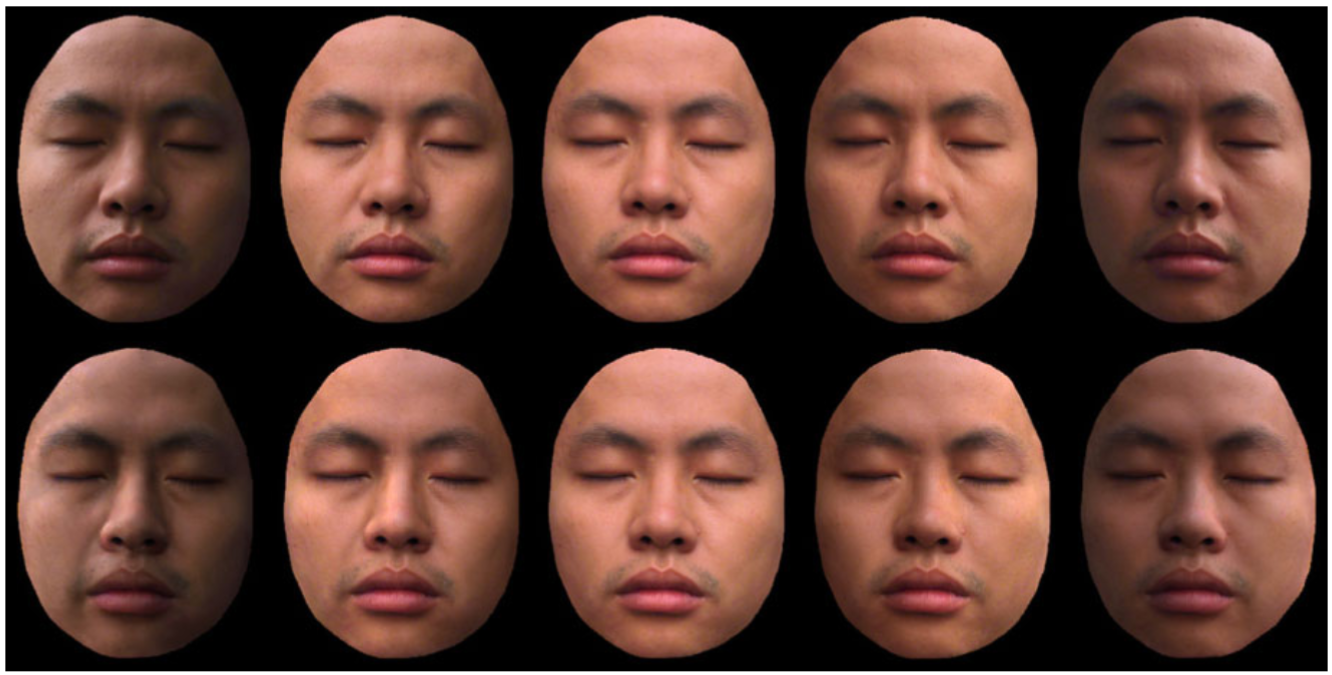
\includegraphics[width=0.85\textwidth]{img/Fig.20.7.png}
    \caption{So sánh kết quả tổng hợp và ảnh thực tế. Hàng trên là ảnh thực tế, hàng dưới là ảnh tổng hợp, ảnh giữa hàng dưới là ảnh đầu vào \cite{wen2003face}.}
    \label{fig:relight_comparison}
\end{figure}

Ngoài ra, phương pháp này còn cho phép chỉnh sửa chiếu sáng bằng cách điều chỉnh trực tiếp các hệ số Spherical Harmonics đã ước lượng. Với mỗi bộ hệ số mới, kỹ thuật ảnh tỷ lệ trong phương trình \eqref{eq:relight_ratio} được áp dụng để tạo ảnh khuôn mặt dưới điều kiện sáng tương ứng. Hình \ref{fig:lighting_editing} trình bày bốn ví dụ chỉnh sửa chiếu sáng: thêm bóng đổ lên một bên mặt, thay đổi sắc độ màu ánh sáng theo hướng, di chuyển vùng sáng chính từ bên này sang bên kia, và kết hợp cả bóng đổ lẫn thay đổi màu sắc. Khả năng tạo dữ liệu huấn luyện đa dạng về chiếu sáng từ phương pháp này có giá trị lớn cho các bài toán phát hiện và nhận dạng khuôn mặt.

\begin{figure}[htbp]
    \centering
    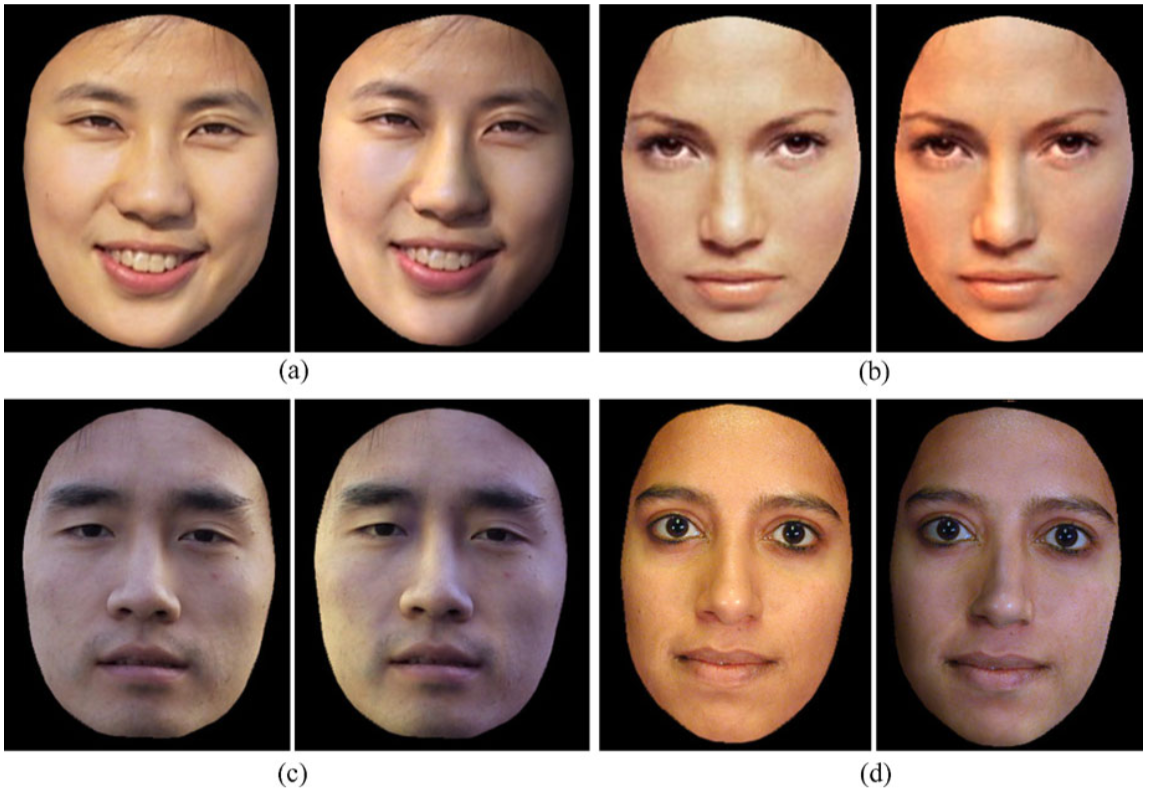
\includegraphics[width=0.85\textwidth]{img/Fig.20.8.png}
    \caption{Chỉnh sửa ánh sáng bằng cách thay đổi hệ số Spherical Harmonics của bản đồ bức xạ. Ảnh bên trái mỗi cặp là ảnh đầu vào, ảnh bên phải là kết quả sau khi chỉnh sửa ánh sáng \cite{wen2003face}.}
    \label{fig:lighting_editing}
\end{figure}

\paragraph{Ứng dụng trong nhận dạng khuôn mặt dưới điều kiện chiếu sáng thay đổi.}
Qing et al. \cite{qing2004face} đã ứng dụng kỹ thuật thay đổi ánh sáng vừa trình bày vào bài toán nhận dạng khuôn mặt dưới các môi trường chiếu sáng khác nhau. Với mỗi ảnh khuôn mặt đầu vào dưới chiếu sáng không xác định, phương pháp này trước tiên tạo ảnh mới dưới chiếu sáng chuẩn hóa, tức là chỉ giữ lại thành phần hằng số $x_{00}$ trong khai triển Spherical Harmonics ở phương trình \eqref{eq:sh_system} và đặt các hệ số còn lại bằng không. Kỹ thuật ảnh tỷ lệ trong phương trình \eqref{eq:relight_ratio} sau đó được sử dụng để sinh ảnh dưới chiếu sáng chuẩn hóa. Quá trình đối sánh ảnh được thực hiện trên các ảnh đã chuẩn hóa chiếu sáng. Thực nghiệm trên cơ sở dữ liệu PIE \cite{sim2003pie} cho thấy tỷ lệ nhận dạng được cải thiện đáng kể sau khi áp dụng kỹ thuật thay đổi ánh sáng.
